\documentclass[11pt,a4paper]{article}

% ===================== PACCHETTI =====================
\usepackage[italian]{babel}
\usepackage[utf8]{inputenc}
\usepackage[T1]{fontenc}
\usepackage[sfdefault,light]{FiraSans}   
\usepackage[scaled=.85]{FiraMono}        
\usepackage[margin=2.5cm]{geometry}
\usepackage{graphicx}
\graphicspath{{immagini/}}
\usepackage{listings}
\usepackage{xcolor}
\usepackage{hyperref}
\usepackage{caption}
\usepackage{fancyhdr}
\usepackage{titlesec}
\usepackage{enumitem}
\usepackage{tikz}
\usepackage{parskip}
\usepackage{dirtree}
\usepackage{tcolorbox}
\tcbuselibrary{listings, skins, breakable}

% ===================== PALETTE COLORI APP =====================
\definecolor{primaryGreen}{HTML}{006D38}
\definecolor{tertiaryBlue}{HTML}{245ABC}
\definecolor{onBackground}{HTML}{161D17}
\definecolor{onSurfaceVariant}{HTML}{3D4A3F}
\definecolor{outlineColor}{HTML}{6D7B6E}
\definecolor{surfaceContainerLow}{HTML}{EEF6EB}
\definecolor{codeString}{HTML}{005229}
% dark theme (blocchi codice)
\definecolor{codeBg}{HTML}{0E150F}
\definecolor{codeText}{HTML}{DDE5DA}
\definecolor{codeKeyword}{HTML}{50E087}
\definecolor{codeComment}{HTML}{9DD3A8}
\definecolor{codeStringDark}{HTML}{B0C6FF}

% ===================== LOGO APP (TikZ) =====================
\newcommand{\LocalShareLogo}[1][1]{%
  \begin{tikzpicture}[scale=#1]
    \begin{scope}
      \clip (0,0) circle (1cm);
      \shade[left color=primaryGreen, right color=tertiaryBlue]
        (-1cm,-1cm) rectangle (1cm,1cm);
    \end{scope}
    \fill[white, opacity=0.95] (-0.214cm, 0) circle (0.388cm);
    \fill[white, opacity=0.95] ( 0.214cm, 0) circle (0.388cm);
  \end{tikzpicture}%
}

% ===================== LINGUAGGIO KOTLIN =====================
\lstdefinelanguage{Kotlin}{
  keywords={fun, val, var, class, object, interface, data, sealed, enum, override,
             suspend, return, if, else, when, for, while, try, catch, throw,
             private, public, internal, protected, companion, by, lazy, true, false, null,
             import, package, is, as, in, out, this, super, init, constructor},
  morecomment=[l]{//},
  morecomment=[s]{/*}{*/},
  morestring=[b]",
  sensitive=true,
}

% ===================== CONFIGURAZIONE CODICE =====================
\lstset{
  basicstyle=\ttfamily\footnotesize,
  breaklines=true,
  keywordstyle=\color{primaryGreen}\bfseries,
  commentstyle=\color{onSurfaceVariant}\itshape,
  stringstyle=\color{codeString},
  showstringspaces=false,
  tabsize=2,
}

\newcommand{\inputcodeblock}[2][Kotlin]{%
  \tcbinputlisting{%
    listing engine=listings,
    listing only, enhanced,
    arc=8pt, colback=codeBg, colframe=tertiaryBlue,
    leftrule=4pt, rightrule=0pt, toprule=0pt, bottomrule=0pt,
    top=6pt, bottom=6pt, left=12pt, right=10pt,
    breakable,
    listing options={%
      language=#1,
      basicstyle=\ttfamily\small\color{codeText},
      breaklines=true,
      keywordstyle=\color{codeKeyword}\bfseries,
      commentstyle=\color{codeComment}\itshape,
      stringstyle=\color{codeStringDark},
      showstringspaces=false, tabsize=2,
    },
    listing file={codice/#2}%
  }%
}

\newtcblisting{codeblock}[1][]{
  listing engine=listings,
  listing only,
  enhanced,
  arc=8pt,
  colback=codeBg,
  colframe=tertiaryBlue,
  leftrule=4pt, rightrule=0pt, toprule=0pt, bottomrule=0pt,
  top=6pt, bottom=6pt, left=12pt, right=10pt,
  breakable,
  listing options={
    basicstyle=\ttfamily\small\color{codeText},
    breaklines=true,
    keywordstyle=\color{codeKeyword}\bfseries,
    commentstyle=\color{codeComment}\itshape,
    stringstyle=\color{codeStringDark},
    showstringspaces=false,
    tabsize=2,
    #1
  }
}

% ===================== STILE SEZIONI =====================
\titleformat{\section}
  {\Large\bfseries\color{tertiaryBlue}}
  {\thesection}{1em}{}
  [\vspace{2pt}{\color{outlineColor}\titlerule[0.4pt]}\vspace{4pt}]

\titleformat{\subsection}
  {\large\bfseries\color{onBackground}}
  {\thesubsection}{1em}{}

\titlespacing*{\section}{0pt}{22pt}{8pt}
\titlespacing*{\subsection}{0pt}{14pt}{4pt}

\addto\captionsitalian{\renewcommand{\refname}{Riferimenti e fonti utilizzate}}

% ===================== METADATI =====================
\newcommand{\nomeProgetto}{LocalShare}
\newcommand{\nomeStudente}{Marco Avogadri}
\newcommand{\matricola}{358105}
\newcommand{\nomeCorso}{Programmazione di sistemi mobili}
\newcommand{\nomeDocente}{Nome Docente}
\newcommand{\nomeUniversita}{Università degli studi di Parma}
\newcommand{\annoAccademico}{2025/2026}

% ===================== INTESTAZIONE/PIEDE PAGINA =====================
\pagestyle{fancy}
\fancyhf{}
\renewcommand{\headrulewidth}{0.4pt}
\renewcommand{\headrule}{{\color{tertiaryBlue}\hrule width\headwidth height\headrulewidth \vskip-\headrulewidth}}
\lhead{\small\color{onSurfaceVariant}Relazione di progetto}
\rhead{\small\color{tertiaryBlue}\textbf{\nomeProgetto}}
\rfoot{\small\color{onSurfaceVariant}\thepage}

\hypersetup{
    colorlinks=true,
    linkcolor=tertiaryBlue,
    urlcolor=tertiaryBlue,
    citecolor=onSurfaceVariant,
    pdftitle={Relazione progetto: \nomeProgetto},
    pdfauthor={\nomeStudente}
}

\begin{document}

% ===================== FRONTESPIZIO =====================
\hypersetup{pageanchor=false}
\begin{titlepage}
    \centering

    {\color{tertiaryBlue}\rule{\textwidth}{2pt}}
    \vspace{0.4cm}

    {\large\color{onBackground}\nomeUniversita \par}
    \vspace{0.15cm}
    {\color{onSurfaceVariant}\nomeCorso \par}

    \vspace{3cm}

    \LocalShareLogo[1.8]
    \vspace{0.6cm}

    {\fontsize{52}{62}\selectfont\color{onBackground}\nomeProgetto \par}
    \vspace{0.5cm}
    {\large\color{onSurfaceVariant} Relazione progetto \par}

    \vfill

    \begin{flushleft}
        {\footnotesize\color{onSurfaceVariant}\MakeUppercase{Studente}}\\[5pt]
        {\large\bfseries\color{onBackground}\nomeStudente}\\[3pt]
        {\small\color{onSurfaceVariant}Matricola:\ \matricola}
    \end{flushleft}

    \vspace{0.8cm}
    
    \vfill

    {\color{outlineColor}\rule{\textwidth}{0.4pt}}
    \vspace{0.4cm}
    {\color{onSurfaceVariant}Anno Accademico\ \annoAccademico}
\end{titlepage}

\hypersetup{pageanchor=true}
\hypersetup{linkcolor=onBackground}
\tableofcontents
\hypersetup{linkcolor=tertiaryBlue}
\newpage

% ===================== CAPITOLI =====================
\section{Introduzione}

\subsection{Scopo dell'applicazione}
LocalShare è una semplice applicazione per scambiare file tra 2 dispositivi in modalità peer to peer.
L'applicativo fornisce quindi la possibilità di vedere i dispositivi nelle vicinanze,
instaurarci una connessione e condividere qualsiasi tipo di file si desidera scambiare.
Nell'applicazione si potrà poi consultare lo storico delle transazioni.


\subsection{Struttura della relazione}
La presente relazione è organizzata come segue:\\ 
il Capitolo~\ref{sec:requisiti} descrive i requisiti e la guida all'installazione;\\ 
il Capitolo~\ref{sec:tecnologie} presenta le tecnologie adottate;\\ 
il Capitolo~\ref{sec:progettazione} illustra le scelte progettuali;\\ 
il Capitolo~\ref{sec:implementazione} entra nel dettaglio dell'implementazione;\\ 
il Capitolo~\ref{sec:funzionamento} mostra il funzionamento dell'applicazione;\\ 
infine il Capitolo~\ref{sec:conclusioni} riporta le conclusioni e i possibili sviluppi futuri.

\section{Requisiti e installazione}
\label{sec:requisiti}

\subsection{Requisiti di sistema}

Questa applicazione è stata realizzata in \textbf{Kotlin},
utilizza un database non relazionale \textbf{MongoDB},
un WebService \textbf{Flask} lato server e un client \textbf{Retrofit}
con \textbf{kotlinx.serialization} per il parsing delle risposte JSON.
Il backend (Flask + MongoDB) è containerizzato tramite \textbf{Docker Compose}.
I requisiti minimi per eseguire l'applicazione sono:

\begin{itemize}[leftmargin=1.2cm]
    \item \textbf{Dispositivo Android con supporto Wi-Fi Direct:} a partire da Android 16 (API Level 36)
    \item \textbf{Android Studio:} IDE per la build e l'installazione dell'app sul dispositivo
    \item \textbf{Docker Desktop:} necessario per avviare i container del backend tramite \texttt{docker compose up}
    \item \textbf{MongoDB Compass} \emph{(opzionale)}: GUI per MongoDB, utile per visualizzare i dati salvati nel database
    \item \textbf{Connessione Internet} \emph{(opzionale)}: richiesta per la sincronizzazione della history e la condivisione di essa con un gruppo di device
\end{itemize}

\subsection{Guida all'installazione}

Il progetto può essere ottenuto scaricando e decomprimendo la cartella \texttt{.zip} fornita, oppure clonando la repository GitHub:

\begin{codeblock}[language=bash]
git clone https://github.com/sonoAv0/LocalShare.git
\end{codeblock}

\subsubsection*{Avvio del backend}

Dalla directory radice del progetto, avviare i container Docker con:

\begin{codeblock}[language=bash]
docker compose up --build
\end{codeblock}

Il comando avvia due container: il WebService Flask (porta \texttt{5000}) e il database MongoDB. Al termine dell'operazione il backend è raggiungibile all'indirizzo \texttt{http://localhost:5000}.

\subsubsection*{Installazione dell'app Android}

Aprire la directory del progetto in Android Studio, collegare un dispositivo Android fisico con il debug USB abilitato oppure avviare un emulatore, quindi eseguire il build e l'installazione tramite il pulsante \emph{Run}. In alternativa, è possibile installare direttamente il file \texttt{localshare.apk} incluso nella directory radice del progetto tramite \texttt{adb}:

\begin{codeblock}[language=bash]
adb install localshare.apk
\end{codeblock}

\subsubsection*{Configurazione dell'indirizzo del backend}

L'URL del backend è definito dalla costante \texttt{BACKEND\_BASE\_URL} nel file \texttt{AppContainer.kt}.

Il valore predefinito \texttt{http://10.0.2.2:5000/} è valido esclusivamente per l'emulatore Android, che utilizza quell'indirizzo speciale per raggiungere il \texttt{localhost} della macchina host. In caso di utilizzo su \textbf{dispositivo fisico}, è necessario sostituirlo con l'indirizzo IP della macchina nella rete locale:

\begin{codeblock}[language=Kotlin]
private const val BACKEND_BASE_URL = "http://192.168.1.X:5000/"
\end{codeblock}

L'IP della macchina host si ottiene eseguendo \texttt{ipconfig} su Windows o \texttt{ip a} su Linux/macOS. Il dispositivo fisico e la macchina host devono essere connessi alla stessa rete.


\section{Tecnologie utilizzate}
\label{sec:tecnologie}

% Per ogni tecnologia, spiega brevemente COSA è e PERCHÉ l'hai scelta
% (non limitarti a elencarla: motiva la scelta rispetto alle alternative).

\subsection{Linguaggi di programmazione}

\begin{itemize}[label={--}, leftmargin=1.2cm]
    \item \textbf{Kotlin}: utilizzato per lo sviluppo dell'applicazione Android.

    \item \textbf{Python}: linguaggio utilizzato per il backend tramite il framework Flask.
\end{itemize}

\subsection{Framework e librerie}

\begin{itemize}[label={--}, leftmargin=1.2cm]
    \item \textbf{Jetpack Compose}: utilizzato per costruire l'interfaccia.

    \item \textbf{Retrofit}: utilizzato per effettuare le chiamate REST al backend Flask.

    \item \textbf{kotlinx.serialization}: utilizzato per il parsing delle risposte JSON del backend.

    \item \textbf{Room}: per la persistenza locale dei dati.

    \item \textbf{WorkManager}: per la sincronizzazione periodica dei dati locali non ancora inviati al backend.

    \item \textbf{Wi-Fi Direct API}: usato per instaurare il collegamento P2P tra i dispositivi.

    \item \textbf{osmdroid}: usata per la visualizzazione della posizione in cui è stata effettuata la transazione all'interno della history.

    \item \textbf{Flask}: framework python usato per la creazione del webservice REST.

    \item \textbf{flask-jwt-extended}: estensione Flask per la gestione dell'autenticazione tramite JSON Web Token (JWT).

    \item \textbf{pymongo}: utilizzato dal backend per leggere e scrivere i dati nel database MongoDB.
\end{itemize}

\subsection{Strumenti di sviluppo}

\begin{itemize}[label={--}, leftmargin=1.2cm]
    \item \textbf{Android Studio}: IDE per lo sviluppo Android.

    \item \textbf{Docker Desktop}: utilizzato per avviare i container del backend.

    \item \textbf{Git / GitHub}: utilizzato per il versionamento del codice.

    \item \textbf{MongoDB Compass}: client di MongoDB per visualizzare il contenuto del database.
\end{itemize}

\section{Progettazione}
\label{sec:progettazione}

\subsection{Architettura generale}

Il sistema è composto da due parti distinte: l'applicazione Android, che funge da client, e un backend REST containerizzato, che gestisce autenticazione, sincronizzazione della history e la logica dei gruppi.

\subsubsection*{Architettura Android -- pattern MVVM}

Il lato Android adotta il pattern \textbf{MVVM} (Model--View--ViewModel). I tre livelli principali sono:

\begin{itemize}[label={--}, leftmargin=1.2cm]
    \item \textbf{UI layer} (\texttt{ui/}): ogni schermata è un \emph{Composable} che osserva uno \texttt{StateFlow} esposto dal proprio ViewModel. Quando lo stato cambia, Compose effettua una recomposition, cambiando la UI in base al suo stato. Il color scheme e la tipografia generale dell'intera UI sono definiti da un tema \textbf{Material 3}.

    \item \textbf{ViewModel} (\texttt{ui/<schermata>/}): raccoglie i dati dalle repository, applica la logica di presentazione e li espone tramite una \texttt{data class} di stato (\texttt{UiState}). Un esempio si può osservare in \texttt{HomeViewModel}, dove vengono esposte le ultime 3 entry della history:

\inputcodeblock{home_viewmodel_recent.kt}

    \item \textbf{Data layer} (\texttt{data/}): espone i dati tramite interfacce di repository, nascondendo alla UI se i dati provengono dal database locale o dal backend.
\end{itemize}

\subsubsection*{Data layer -- struttura a strati}

Il data layer è organizzato in tre sotto-moduli:

\begin{itemize}[label={--}, leftmargin=1.2cm]
    \item \texttt{data/local/db/}: database SQLite creato con Room per la persistenza locale dei dati. E' il metodo primario di persistenza dell'applicazione. 
    \item \texttt{data/remote/}: interfaccia Retrofit \texttt{LocalShareApi} con le chiamate REST per la comunicazione con il web service Flask, il quale persiste i dati su un database non relazionale MongoDB. 
    \item \texttt{data/p2p/}: gestione della connessione Wi-Fi Direct e del trasferimento file con protocollo TCP.
\end{itemize}

\subsubsection*{Comunicazione con il backend}

La sincronizzazione con il backend è \textbf{opzionale}: l'app funziona in modo autonomo anche senza connessione, poiché l'identità del dispositivo è un UUID generato localmente alla prima installazione tramite \texttt{DeviceIdProvider}, senza bisogno di contattare alcun server. Il backend viene coinvolto solo per la sincronizzazione della history e la condivisione tramite gruppi.

Quando la sincronizzazione è abilitata, le chiamate REST sono effettuate tramite \textbf{Retrofit}, con \textbf{kotlinx.serialization} come converter per il parsing JSON.
L'autenticazione avviene tramite JWT: l'app registra il proprio UUID sul backend e ottiene un token, che viene salvato nelle \texttt{Shared\-Preferences}; per far sì che ogni chiamata abbia nell'header il token, viene utilizzato un interceptor:

\inputcodeblock{okhttp_jwt_interceptor.kt}

La repository \texttt{SyncedHistoryRepository} si occupa della sincronizzazione tra la repository locale e quella backend, dando precedenza alla persistenza locale: ogni trasferimento viene prima salvato nel database Room, poi si tenta l'invio al backend. Se la rete non è disponibile, un \texttt{WorkManager} si occuperà di ritentantare la sincronizzazione una volta che il dispositivo ritornerà connesso.

\subsection{Struttura dei dati / Database}

L'applicazione utilizza due livelli di persistenza distinti: un database locale sul dispositivo Android (metodo principale e sempre utilizzato) e un database remoto sul backend (secondario e utilizzato secondo le preferenze dell'utente).

\subsubsection*{Persistenza locale -- Room (SQLite)}

Il database locale necessita di una sola tabella contenente le entry che costituiscono la history delle transazioni di un utente: \texttt{history}, mappata dalla \texttt{data class} \texttt{HistoryEntity}:

\begin{itemize}[label={--}, leftmargin=1.2cm]
    \item \texttt{transferId}: UUID che identifica univocamente il trasferimento; è la chiave condivisa con il backend.
    \item \texttt{peerDeviceId}: UUID del dispositivo con cui è avvenuto lo scambio.
    \item \texttt{fileName}: nome del file trasferito.
    \item \texttt{sizeBytes}: dimensione del file trasferito.
    \item \texttt{direction}: enum \texttt{SENT} / \texttt{RECEIVED} per identificare i file trasferiti da quelli ricevuti.
    \item \texttt{timestampMillis}: timestamp della transazione.
    \item \texttt{latitude}, \texttt{longitude}: campi opzionali che salvano la posizione in cui il trasfermento è avvenuto.
    \item \texttt{isSynced}: flag presente solamente nel DB locale che indica se l'entry è già stata inviata al backend.
\end{itemize}

\subsubsection*{Persistenza remota -- MongoDB}

Nel backend sono presenti 3 collection MongoDB:

\begin{itemize}[label={--}, leftmargin=1.2cm]
    \item \texttt{users}: un documento per dispositivo registrato, contenente lo \texttt{user\_id} (UUID) e il timestamp \texttt{created\_at}.

    \item \texttt{transfers}: un documento per trasferimento, ha gli stessi campi di \texttt{HistoryEntity} locale (escluso \texttt{isSynced}) più \texttt{user\_id} per indicarne il proprietario e \texttt{group\_code} opzionale.

    \item \texttt{groups}: un documento per gruppo, con un codice alfanumerico di 6 caratteri generato casualmente e un array \texttt{members} contenente gli \texttt{user\_id} dei partecipanti. Una volta entrato in un gruppo, un dispositivo vedrà nella sua sezione history le transazioni degli altri dispositivi del gruppo. 
\end{itemize}

\subsection{Scelte progettuali}

\subsubsection*{Design pattern}

\begin{itemize}[label={--}, leftmargin=1.2cm]
    \item \textbf{Repository pattern}: Ogni repository (locale e backend) è nascosta grazie ad un'interfaccia: \texttt{DeviceRepository} e \texttt{HistoryRepository}. Grazie a questo layer di astrazione, i viewModel istanziano l'interfaccia e quindi non sanno i dettagli del database su cui stanno lavorando.  

    \item \textbf{Strategy pattern}: \texttt{P2pManager} e \texttt{TransferManager} sono interfacce con implementazioni concrete (\texttt{WifiDirectP2pManager}, \texttt{SocketTransferManager}) iniettate da \texttt{AppContainer}. Questo layer di astrazione nasconde l'implementazione della metodologia di trasferimento dati dalla logica di business. Se per esempio si volesse implementare un nuovo metodo di trasferimento (es. Bluetooth)
    per applicarla alla logica di business basterebbe cambiare l'injection in \texttt{AppContainer}. 

    \item \textbf{Singleton}: Nel progetto si trovano due \texttt{object} Kotlin. \texttt{TransferSessionState} espone un flag condiviso \texttt{isTransferring} usato per coordinare \texttt{Incoming\-Transfer\-Watcher} e \texttt{Transfer\-Foreground\-Service} (il suo ruolo è approfondito nella sezione \hyperref[subsec:broadcast]{BroadcastReceiver}). \texttt{AppContainer} è anch'esso un singleton, descritto successivamente.

    \item \textbf{Factory Method}: ogni schermata definisce una \texttt{viewModelFactory} che incapsula la logica di costruzione del proprio ViewModel, separandola dal codice che lo utilizza. Questo è necessario perché Compose non può costruire ViewModel con parametri arbitrari tramite il meccanismo di default; la factory fornisce al sistema le istruzioni su come creare l'istanza. Un esempio concreto in \texttt{HomeScreen}:

\begin{codeblock}[language=Kotlin]
private val HomeViewModelFactory = viewModelFactory {
    initializer {
        HomeViewModel(
            AppContainer.deviceIdProvider,
            AppContainer.deviceRepository,
            AppContainer.historyRepository,
        )
    }
}
\end{codeblock}

    \item \textbf{Dependency injection manuale}: \texttt{AppContainer} funge da injector, istanziando tutte le dipendenze principali (repository, client HTTP, database, manager P2P) e le fornisce ai ViewModel tramite le factory descritte sopra.
\end{itemize}

\subsubsection*{Composable}

Un \textbf{Composable} è una funzione Kotlin annotata con \texttt{@Composable} che descrive una porzione dell'interfaccia utente in modo dichiarativo: invece che essere modifiata esplicitamente, la view intercetta e cambia a seconda dello stato corrente attraverso una recomposition.

Lo stato può essere gestito a due livelli distinti:

Lo \textbf{stato di ViewModel} (\texttt{StateFlow}) è usato per dati che devono sopravvivere alle recomposition, alle rotazioni di schermo e che provengono dalla logica di business.

Lo \textbf{stato interno al Composable} viene gestito con \texttt{remember \{ mutableStateOf(...) \}}. E' usato per dati esclusivamente visivi di cui non è richiesta la sopravvivenza alla recomposition. Un esempio concreto all'interno del progetto è il seguente:

\begin{itemize}[label={--}, leftmargin=1.2cm]
    \item le \texttt{HistoryCard} all'interno della schermata di History usano \texttt{var expanded by remember \{ mutableStateOf(false) \}} per tracciare il loro stato, che può essere espanso o collassato.
\end{itemize}

\begin{figure}[h]
    \centering
    \begin{minipage}[c]{0.42\textwidth}
        \centering
        
\includegraphics[width=\textwidth]{card_history_collapsed.png}
    \end{minipage}
    \hfill
    \begin{minipage}[c]{0.42\textwidth}
        \centering
        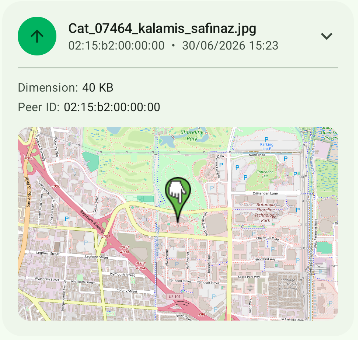
\includegraphics[width=\textwidth]{card_history_expanded.png}
    \end{minipage}
    \caption{HistoryCard collassata (sinistra) ed espansa (destra)}
\end{figure}

\subsubsection*{Coroutines}

Le operazioni asincrone (chiamate di rete, I/O su disco, trasferimento file) sono gestite tramite coroutine.
Nei ViewModel le coroutine vengono lanciate in \texttt{viewModelScope}, che le annulla automaticamente quando il ViewModel viene distrutto.\\
Un utilizzo più avanzato delle coroutine si ha nella funzione \texttt{observePeers} utilizzata al momento della discovery dei dispositivi nelle vicinanze dove l'API di WiFi-Direct, basata su callback, viene adattata a un \texttt{Flow} Kotlin:

\begin{codeblock}[language=Kotlin]
override fun observePeers(): Flow<List<PeerDevice>> = callbackFlow {
    val receiver = object : BroadcastReceiver() {
        override fun onReceive(ctx: Context, intent: Intent) {
            if (intent.action == WifiP2pManager.WIFI_P2P_PEERS_CHANGED_ACTION)
                requestPeers()
        }
    }
    ContextCompat.registerReceiver(context, receiver, IntentFilter(...), ...)
    awaitClose { context.unregisterReceiver(receiver) }
}
\end{codeblock}

\subsubsection*{BroadcastReceiver e Wi-Fi Direct}%
\label{subsec:broadcast}

L'API Wi-Fi Direct notifica gli eventi di rete tramite \textbf{Broad\-cast\-Receiver}. In \texttt{Wifi\-Direct\-P2p\-Manager} vengono registrati due receiver:

\begin{itemize}[label={--}, leftmargin=1.2cm]
    \item \texttt{WIFI\_P2P\_PEERS\_CHANGED\_ACTION}: inviato dal sistema quando la lista dei dispositivi vicini cambia; alla ricezione viene richiesta la lista aggiornata e inviata al Flow.
    \item \texttt{WIFI\_P2P\_CONNECTION\_CHANGED\_ACTION}: inviato quando lo stato della connessione P2P cambia; alla ricezione vengono richieste le informazioni sul gruppo formato (indirizzo del group owner, ruolo del dispositivo).
\end{itemize}

\texttt{Incoming\-Transfer\-Watcher} osserva il Flow di \texttt{observeConnectionInfo()} in una coroutine con scope dedicato e, quando rileva una nuova connessione P2P, avvia il \texttt{Transfer\-Foreground\-Service} in modalità ricezione. Tuttavia il broadcast \texttt{WIFI\_P2P\_CONNECTION\_CHANGED\_ACTION} viene ricevuto da entrambi i dispositivi coinvolti nella connessione, incluso il mittente. Per evitare che il mittente avvii erroneamente una sessione di ricezione, \texttt{Incoming\-Transfer\-Watcher} controlla il flag \texttt{Transfer\-Session\-State.isTransferring} prima di procedere: se il dispositivo ha già avviato un trasferimento, il flag è \texttt{true} e il servizio non viene avviato.

\subsubsection*{Foreground Service}

Il trasferimento file avviene al di fuori del ciclo di vita di Activity e ViewModel, in un \textbf{Foreground Service} (\texttt{TransferForegroundService}). Questa scelta è necessaria perché il trasferimento può durare diversi secondi e deve continuare anche se l'utente naviga fuori dalla schermata. Android richiede che un servizio in primo piano mostri una \textbf{notifica persistente} per tutta la durata dell'operazione, in modo che l'utente sia consapevole dell'attività in corso.

\section{Implementazione}
\label{sec:implementazione}

\subsection{Struttura del codice}

Il progetto è suddiviso in due componenti principali: l'applicazione Android e il backend Flask.

\subsubsection*{Applicazione Android}

\noindent\begin{minipage}{\textwidth}
\dirtree{%
.1 localshare/.
.2 MainActivity.kt.
.2 data/.
.3 AppContainer.kt.
.3 local/.
.4 DeviceIdProvider.kt.
.4 BackendPreferences.kt.
.4 db/.
.5 HistoryEntity.kt.
.5 HistoryDao.kt.
.5 LocalShareDatabase.kt.
.3 remote/.
.4 LocalShareApi.kt.
.4 ApiModels.kt.
.4 AuthInterceptor.kt.
.3 p2p/.
.4 P2pManager.kt.
.4 WifiDirectP2pManager.kt.
.4 TransferManager.kt.
.4 SocketTransferManager.kt.
.4 IncomingTransferWatcher.kt.
.3 repository/.
.4 HistoryRepository.kt.
.4 LocalHistoryRepository.kt.
.4 SyncedHistoryRepository.kt.
.4 DeviceRepository.kt.
.4 BackendDeviceRepository.kt.
.2 service/.
.3 TransferForegroundService.kt.
.3 SyncWorker.kt.
.2 ui/.
.3 home/.
.3 discovery/.
.3 history/.
.3 settings/.
.3 navigation/.
.3 theme/.
}
\end{minipage}

\begin{itemize}[label={--}, leftmargin=1.2cm]
    \item \texttt{data/local/}: persistenza locale tramite Room e preferenze in \texttt{Shared\-Preferences}.
    \item \texttt{data/remote/}: interfaccia Retrofit e modelli di serializzazione per le chiamate REST.
    \item \texttt{data/p2p/}: gestione della connessione Wi-Fi Direct e del trasferimento file via socket TCP.
    \item \texttt{data/repository/}: repository che astraggono le sorgenti dati; \texttt{Synced\-His\-to\-ry\-Re\-po\-si\-to\-ry} combina locale e remoto.
    \item \texttt{service/}: \texttt{TransferForegroundService} mantiene attivo il trasferimento in background; \texttt{SyncWorker} ritenta la sincronizzazione quando torna la connessione.
    \item \texttt{ui/}: schermate e ViewModel organizzati per funzionalità; \texttt{theme/} contiene la palette e la tipografia Material~3.
\end{itemize}

\subsubsection*{Backend Flask}

\dirtree{%
.1 backend/.
.2 run.py.
.2 app/.
.3 \_\_init\_\_.py.
.3 config.py.
.3 routes/.
.4 auth.py.
.4 history.py.
.4 groups.py.
}

\begin{itemize}[label={--}, leftmargin=1.2cm]
    \item \texttt{run.py}: punto di ingresso dell'applicazione Flask.
    \item \texttt{app/\_\_init\_\_.py}: inizializza l'app, configura JWT e la connessione MongoDB.
    \item \texttt{routes/auth.py}: endpoint di registrazione e login tramite UUID.
    \item \texttt{routes/history.py}: endpoint per registrare e recuperare i trasferimenti.
    \item \texttt{routes/groups.py}: endpoint per creare e unirsi a un gruppo.
\end{itemize}

\subsection{Funzionalità principali}

Le funzionalità dell'applicazione possono essere elencate seguendo 3 macrocategorie:
\begin{itemize}[label={--}, leftmargin=1.2cm]
    \item \texttt{Connessione con Wi-Fi Direct}
    \item  \texttt{Trasferimento di file tramite socket TCP}
    \item \texttt{Persistenza dei dati (locali/su backend)}
\end{itemize}

\subsubsection*{Connessione Wi-Fi Direct}

La connessione tra dispositivi è gestita da \texttt{WifiDirectP2pManager}, che fa da wrapper attorno alle API di sistema \texttt{WifiP2pManager}. Il flusso principale è il seguente:

\begin{enumerate}[leftmargin=1.4cm]
    \item \textbf{Discovery}: \texttt{startDiscovery()} avvia la scansione dei dispositivi vicini tramite \texttt{manager.\allowbreak discoverPeers()}. Come spiegato precedentemente, ogni cambiamento nella lista dei peer disponibili viene segnalato dal broadcast \texttt{WIFI\_P2P\_\allowbreak PEERS\_\allowbreak CHANGED\_\allowbreak ACTION}; questo all'interno del contesto di coroutine \texttt{callbackFlow} che lo intercetta e richiede la lista aggiornata, ritornando una \texttt{Flow<List<\allowbreak PeerDevice>>}.

    \pagebreak
    \item \textbf{Connessione}: in questa fase viene stabilito da Wi-Fi direct quale dispositivo sarà il group owner (il server) e quale il client formando il gruppo P2P. Anche in questo caso il metodo \texttt{connect()} dell'API viene adattato perchè basato su callback, questa volta usando il blocco \texttt{suspendCancellableCoroutine}:
\end{enumerate}

\inputcodeblock{wifidirect_connect.kt}

Quando \texttt{connet()} ritorna success, il sistema invia il broadcast \texttt{WIFI\_P2P\_\allowbreak CONNECTION\_\allowbreak CHANGED\_\allowbreak ACTION}, ma il gruppo non si sarà ancora formato. Subito dopo quindi \texttt{observeConnectionInfo()} lo intercetta e restituisce le informazioni sul gruppo P2P formato: l'indirizzo IP del group owner e il ruolo del dispositivo (owner o client), che vengono passate al \texttt{Transfer\-Foreground\-Service} per avviare il trasferimento:

\inputcodeblock{group_creation.kt}
{\small\color{onSurfaceVariant}\itshape\centering Dopo la connessione prova per 30 secondi a controllare che il gruppo sia creato\par}
\vspace{4pt}

\subsubsection*{Trasferimento file via socket TCP}

Una volta ottenute le informazioni di connessione, il trasferimento avviene tramite socket TCP sulla porta \texttt{8988}. L'apertura del socket segue ruoli distinti in base al ruolo nel gruppo P2P:

\inputcodeblock{socket_open.kt}

Il \emph{group owner} funge da server: apre un \texttt{ServerSocket} e attende la connessione in ingresso con \texttt{accept()}. Il \emph{client} si connette attivamente all'indirizzo IP del group owner. 

Il protocollo di trasferimento dei file funziona attraverso 2 stream: il mittente scrive su un \texttt{DataOutputStream} il nome del file, la dimensione in byte e il contenuto del file tramite \texttt{copyTo}. Il ricevente legge gli stessi campi nello stesso ordine e salva il file nella directory esterna dell'app:

\inputcodeblock{send_file.kt}
{\small\color{onSurfaceVariant}\itshape\centering Metodo di invio file, il metodo di ricezione è speculare\par}
\vspace{4pt}

\subsubsection*{Persistenza dei dati}

\subsubsection*{SQLite con Android Room}

Al termine di ogni trasferimento, \texttt{Transfer\-Foreground\-Service} chiama il metodo \texttt{\allowbreak recordTransfer()} di \texttt{history\-Repository}, che in \texttt{Local\-History\-Repository} genera un UUID e lo inserisce nella tabella \texttt{history} tramite il DAO.

\inputcodeblock{local_record_transfer.kt}

\subsubsection*{Backend con Flask e MongoDB}

Se l'utente decide di attivare la sincronizzazione, le entry precedentemente salvate in locale saranno sincronizzate su MongoDB e quelle create successivamente saranno salvate su entrambi i DB. La politica di persistenza è però \texttt{local first}: il metodo di salvataggio principale e garantito resta il DB su Room e successivamente viene tentato sul backend:

\inputcodeblock{synced_record_transfer.kt}

Viene inoltre utilizzato un \texttt{SyncWorker} tramite \texttt{WorkManager} per tutte le chiamate REST al backend fallite (mancanza di connessione / errori del server), e una volta tornata la connessione tenta la sync verrà ritentata la sincronizzazione di tutte quelle entry locali con il flag \texttt{isSynced = false}  

La stessa logica si applica ai gruppi: quando un dispositivo entra in un gruppo, \texttt{associate\-To\-Group()} carica sul backend tutte le entry locali esistenti con il codice del gruppo, rendendole visibili agli altri membri.

\subsubsection*{Schermate e ViewModel}

Ogni schermata (\texttt{HomeScreen}, \texttt{DiscoveryScreen}, \texttt{HistoryScreen}, \texttt{SettingsScreen}) è un Composable associato al proprio ViewModel, creato tramite una \texttt{viewModelFactory} come descritto nella sezione~\ref{sec:progettazione}. I ViewModel espongono lo stato tramite \texttt{StateFlow} e le schermate si aggiornano tramite recomposition. La navigazione tra schermate è gestita da \texttt{NavHost} in \texttt{navigation/}.

\pagebreak


\section{Funzionamento dell'applicazione}
\label{sec:funzionamento}

\subsection{Schermata principale}

L'applicazione all'avvio mostrerà la \textbf{Home Screen}, che fornisce un collegamento diretto a tutte le funzionalità offerte dall'app.

La schermata è suddivisa in tre parti principali: la prima mostra il \textbf{Device ID} del dispositivo, al lato l'icona in verde conferma la corretta autenticazione del dispositivo; 

poco sotto ci sono i bottoni di navigazione per le schermate dell'app: il primo in verde per iniziare un trasfermento porterà alla schermata dove inizierà la discovery dei dispositivi circostanti,

i due tasti sotto portano invece portano rispettivamente alla history delle transazioni e alle opzioni, dove l'utente ha la possibilità di abilitare il synch con il backend e gestire i gruppi.

nella parte sottostante sono mostrate le ultime tre transazioni effettuate, ciascuna mostrata in una card con il nome del file, la dimensione, la direzione (invio o ricezione) e il timestamp.

\vspace{12pt}
\begin{figure}[h]
    \centering
    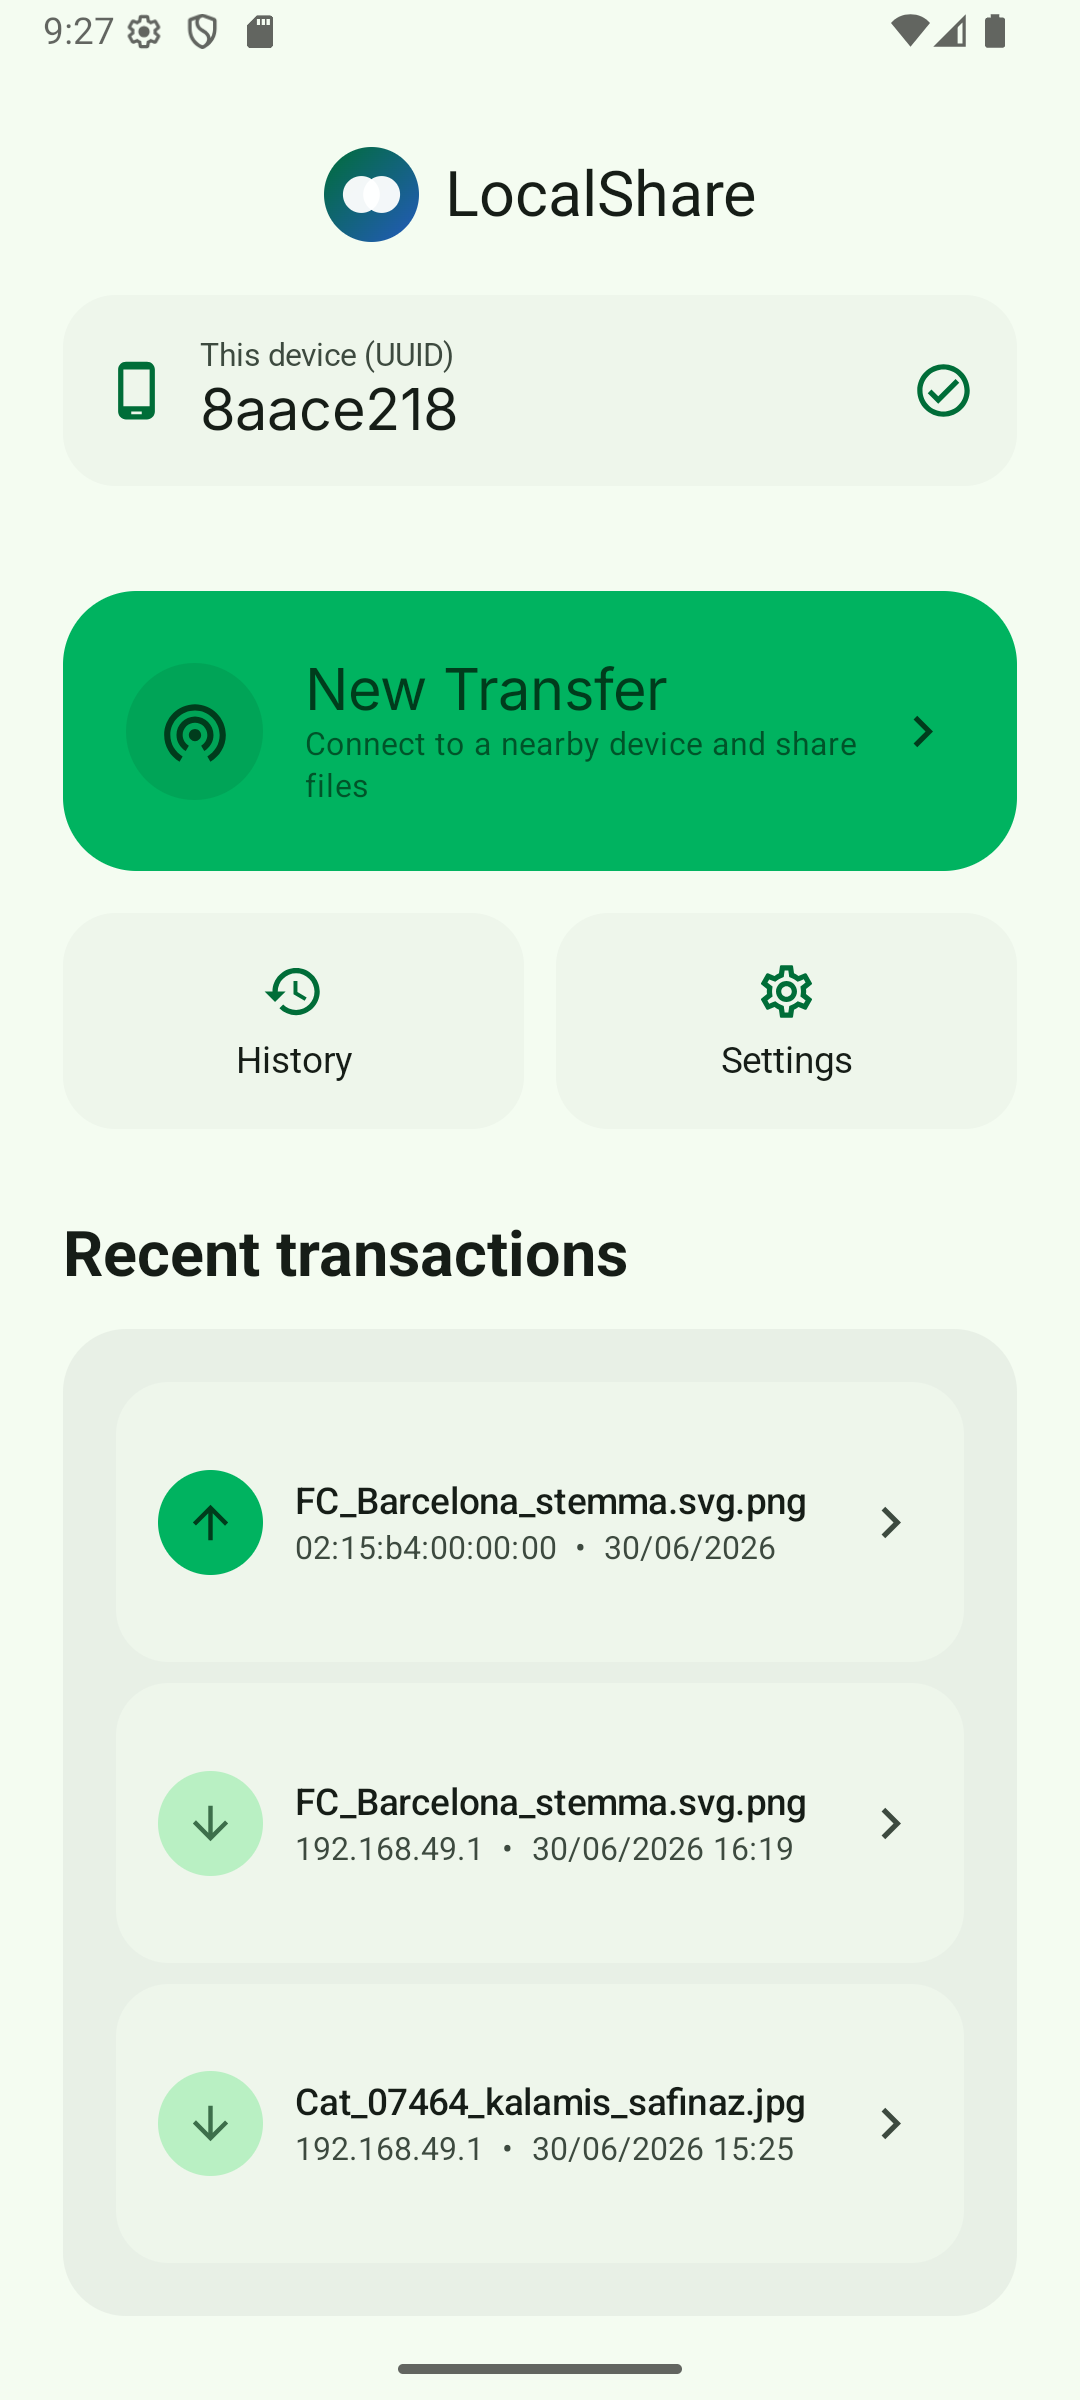
\includegraphics[width=0.42\textwidth]{home_page.png}
    \caption{Home Screen con le ultime transazioni recenti}
    \label{fig:home}
\end{figure}

\subsection{Navigazione}

\subsubsection*{Discovery e invio file}

Premendo il tasto verde nella Home l'utente accede alla \textbf{Discovery Screen}. L'app avvia automaticamente la scansione Wi-Fi Direct e mostra i dispositivi rilevati nelle vicinanze. Per avviare un trasferimento l'utente seleziona prima il dispositivo destinatario e poi sceglie il file dal file picker di sistema; a quel punto inizierà il traferimento, facendo comparire la notifica persistente di avanzamento.

\vspace{12pt}
\begin{figure}[h]
    \centering
    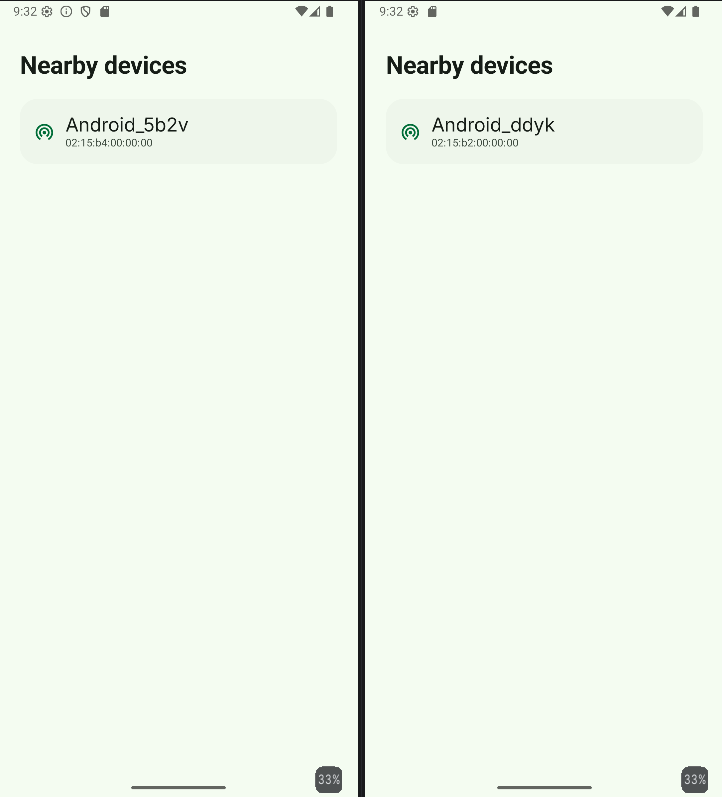
\includegraphics[width=0.65\textwidth]{pairing_page.png}
    \caption{Discovery Screen con i dispositivi rilevati nelle vicinanze}
    \label{fig:discovery}
\end{figure}

\pagebreak
\subsubsection*{History}

La \textbf{History Screen} elenca tutte le transazioni registrate, sia locali che sincronizzate dal gruppo. Ogni \texttt{HistoryCard} è collassabile: inizialmente mostra le info principali come nome del file e il timestamp; espandendola compaiono anche il Device ID del peer e, se disponibile, la posizione in cui è avvenuto il trasferimento.

\vspace{12pt}
\begin{figure}[h]
    \centering
    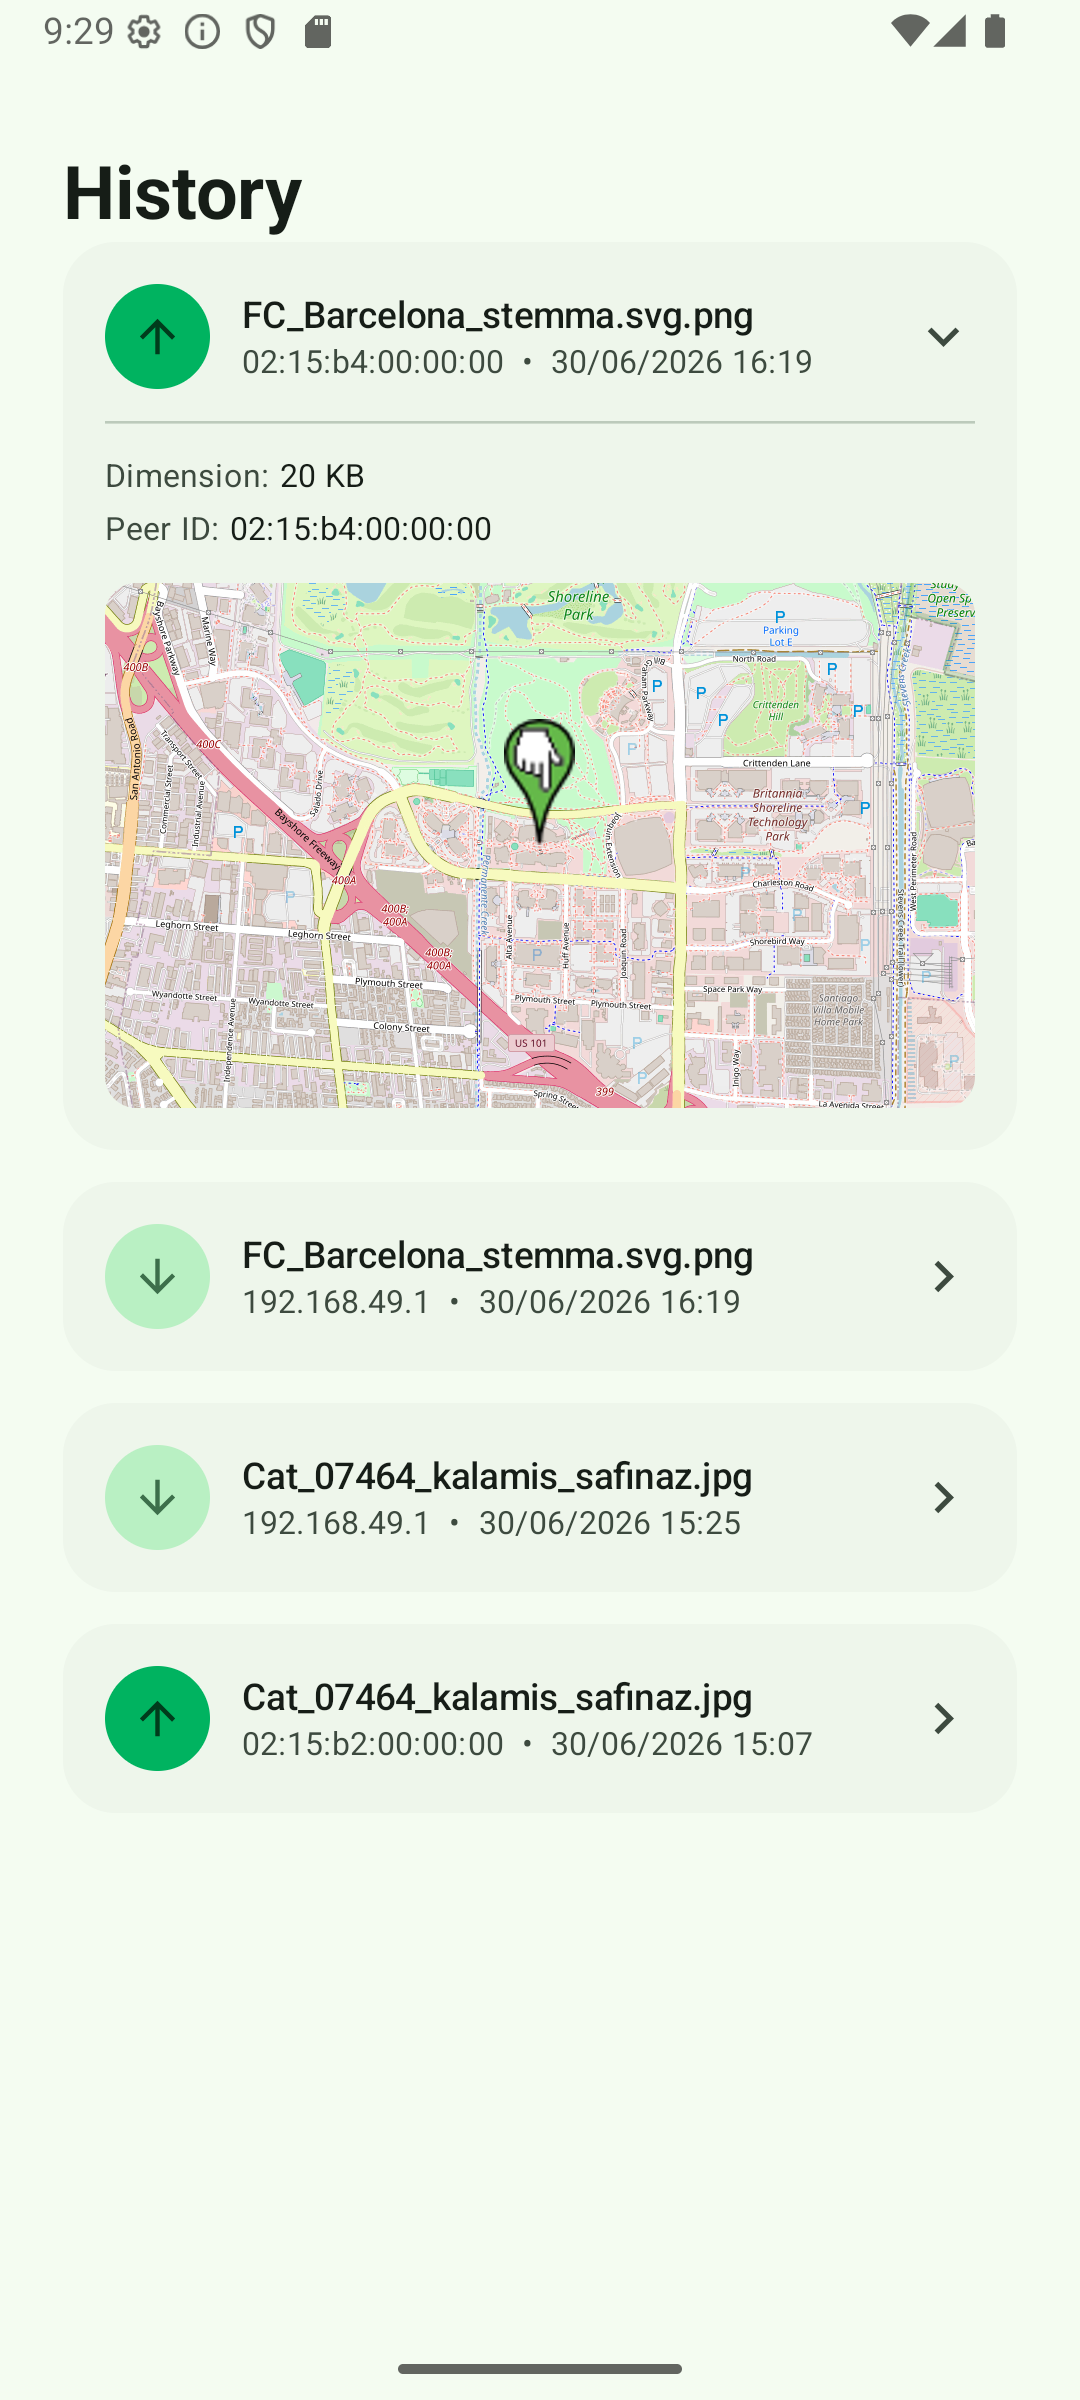
\includegraphics[width=0.42\textwidth]{history_page.png}
    \caption{History Screen con le transazioni registrate}
    \label{fig:history}
\end{figure}

\pagebreak
\subsubsection*{Impostazioni e gruppi}

La \textbf{Settings Screen} permette di abilitare la sincronizzazione con il backend e di gestire i gruppi. Attivandolo, l'app registra il dispositivo sul backend ottenendo il token. Nella sezione gruppi l'utente può creare un nuovo gruppo oppure unirsi a uno esistente inserendo il codice; al join, tutte le entry locali vengono caricate sul backend con il codice del gruppo, rendendole visibili agli altri membri.

\vspace{12pt}
\begin{figure}[h]
    \centering
    \begin{minipage}[t]{0.42\textwidth}
        \centering
        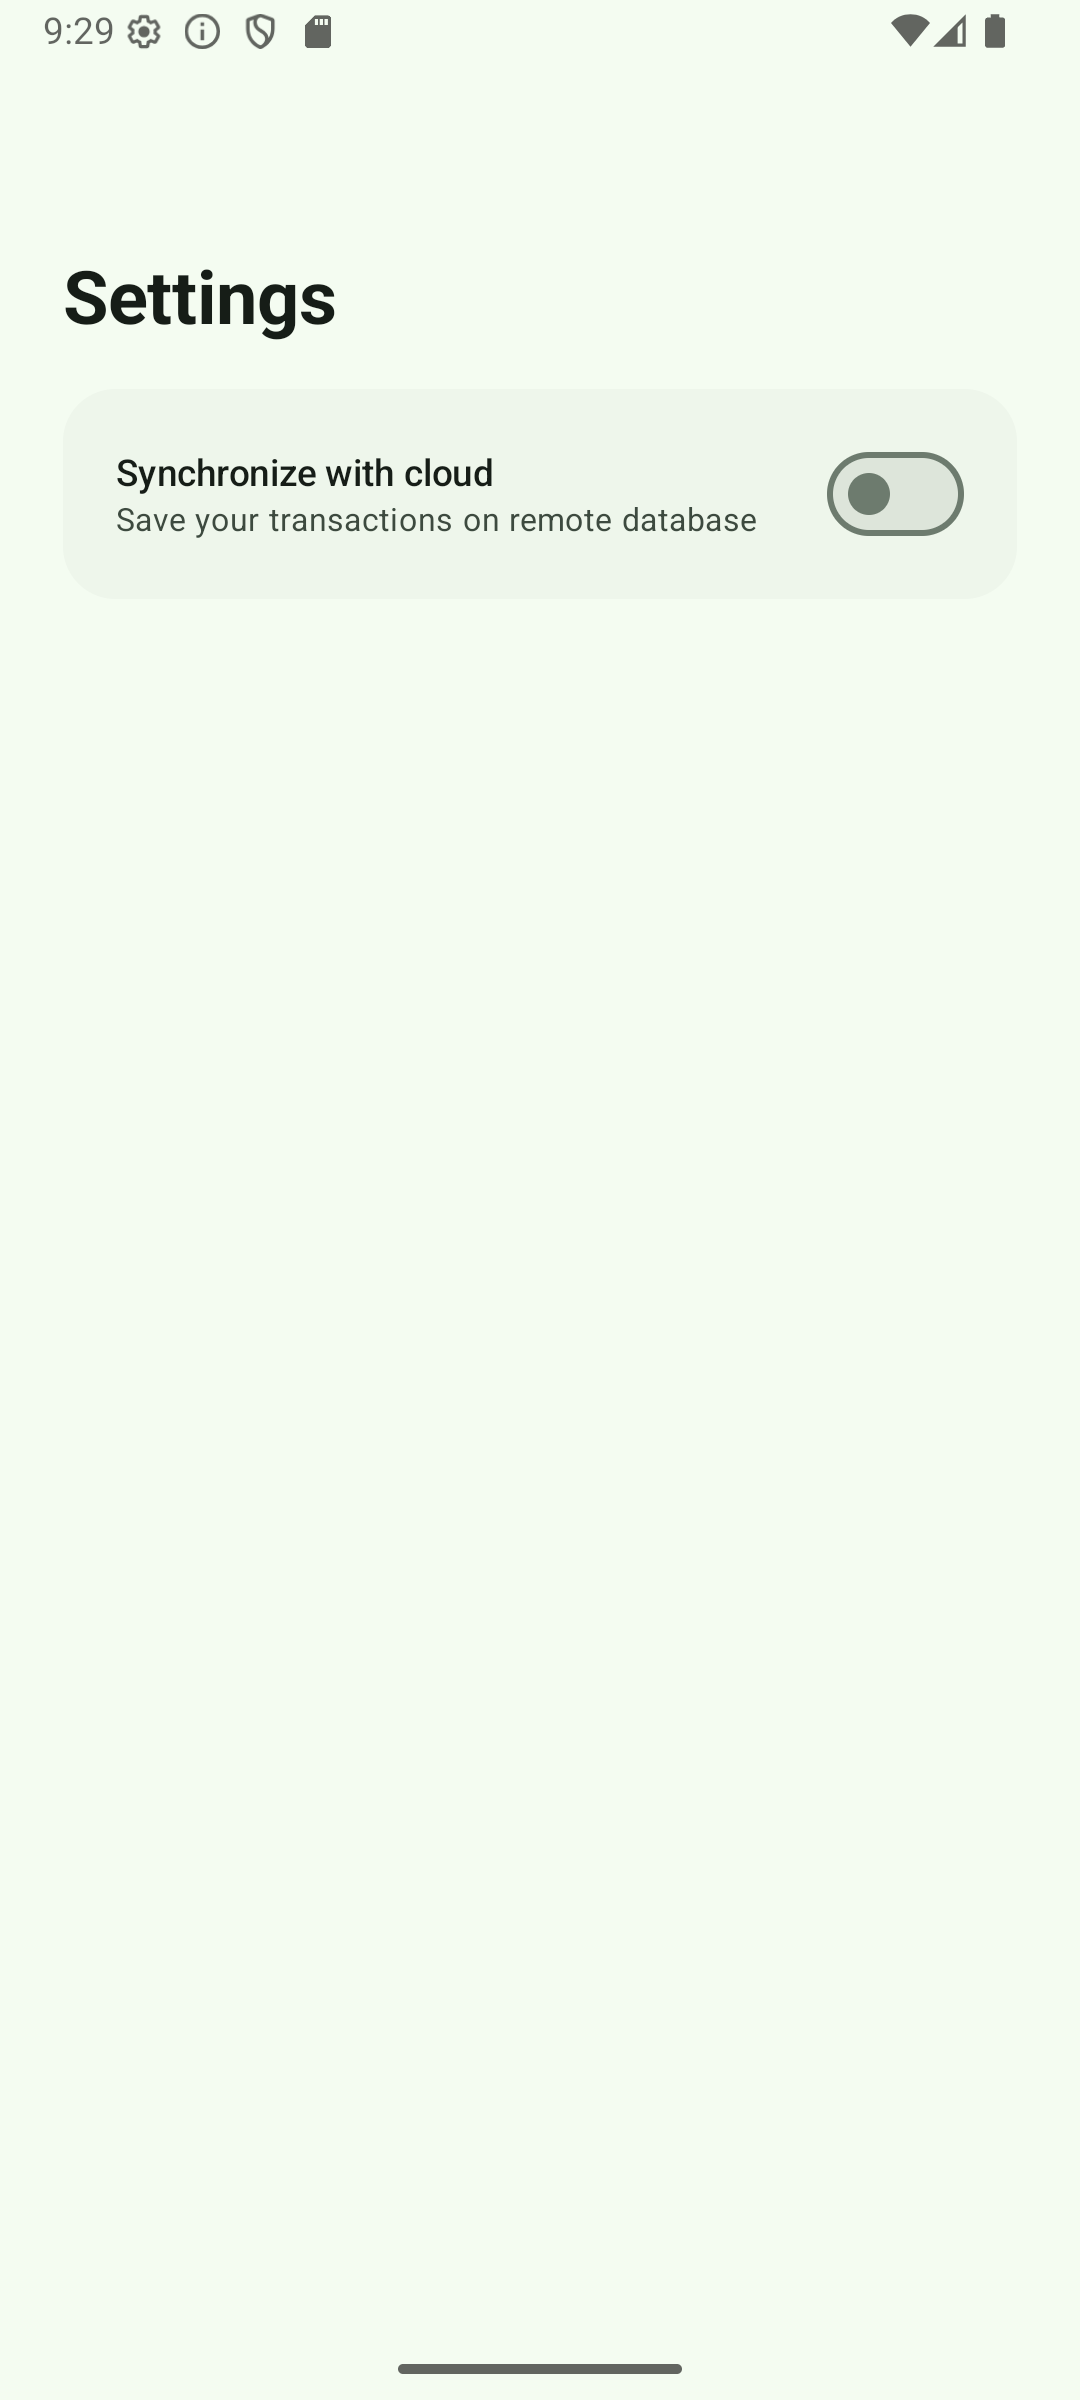
\includegraphics[width=\textwidth]{settings_page.png}
        \caption{Settings Screen}
        \label{fig:settings}
    \end{minipage}
    \hfill
    \begin{minipage}[t]{0.42\textwidth}
        \centering
        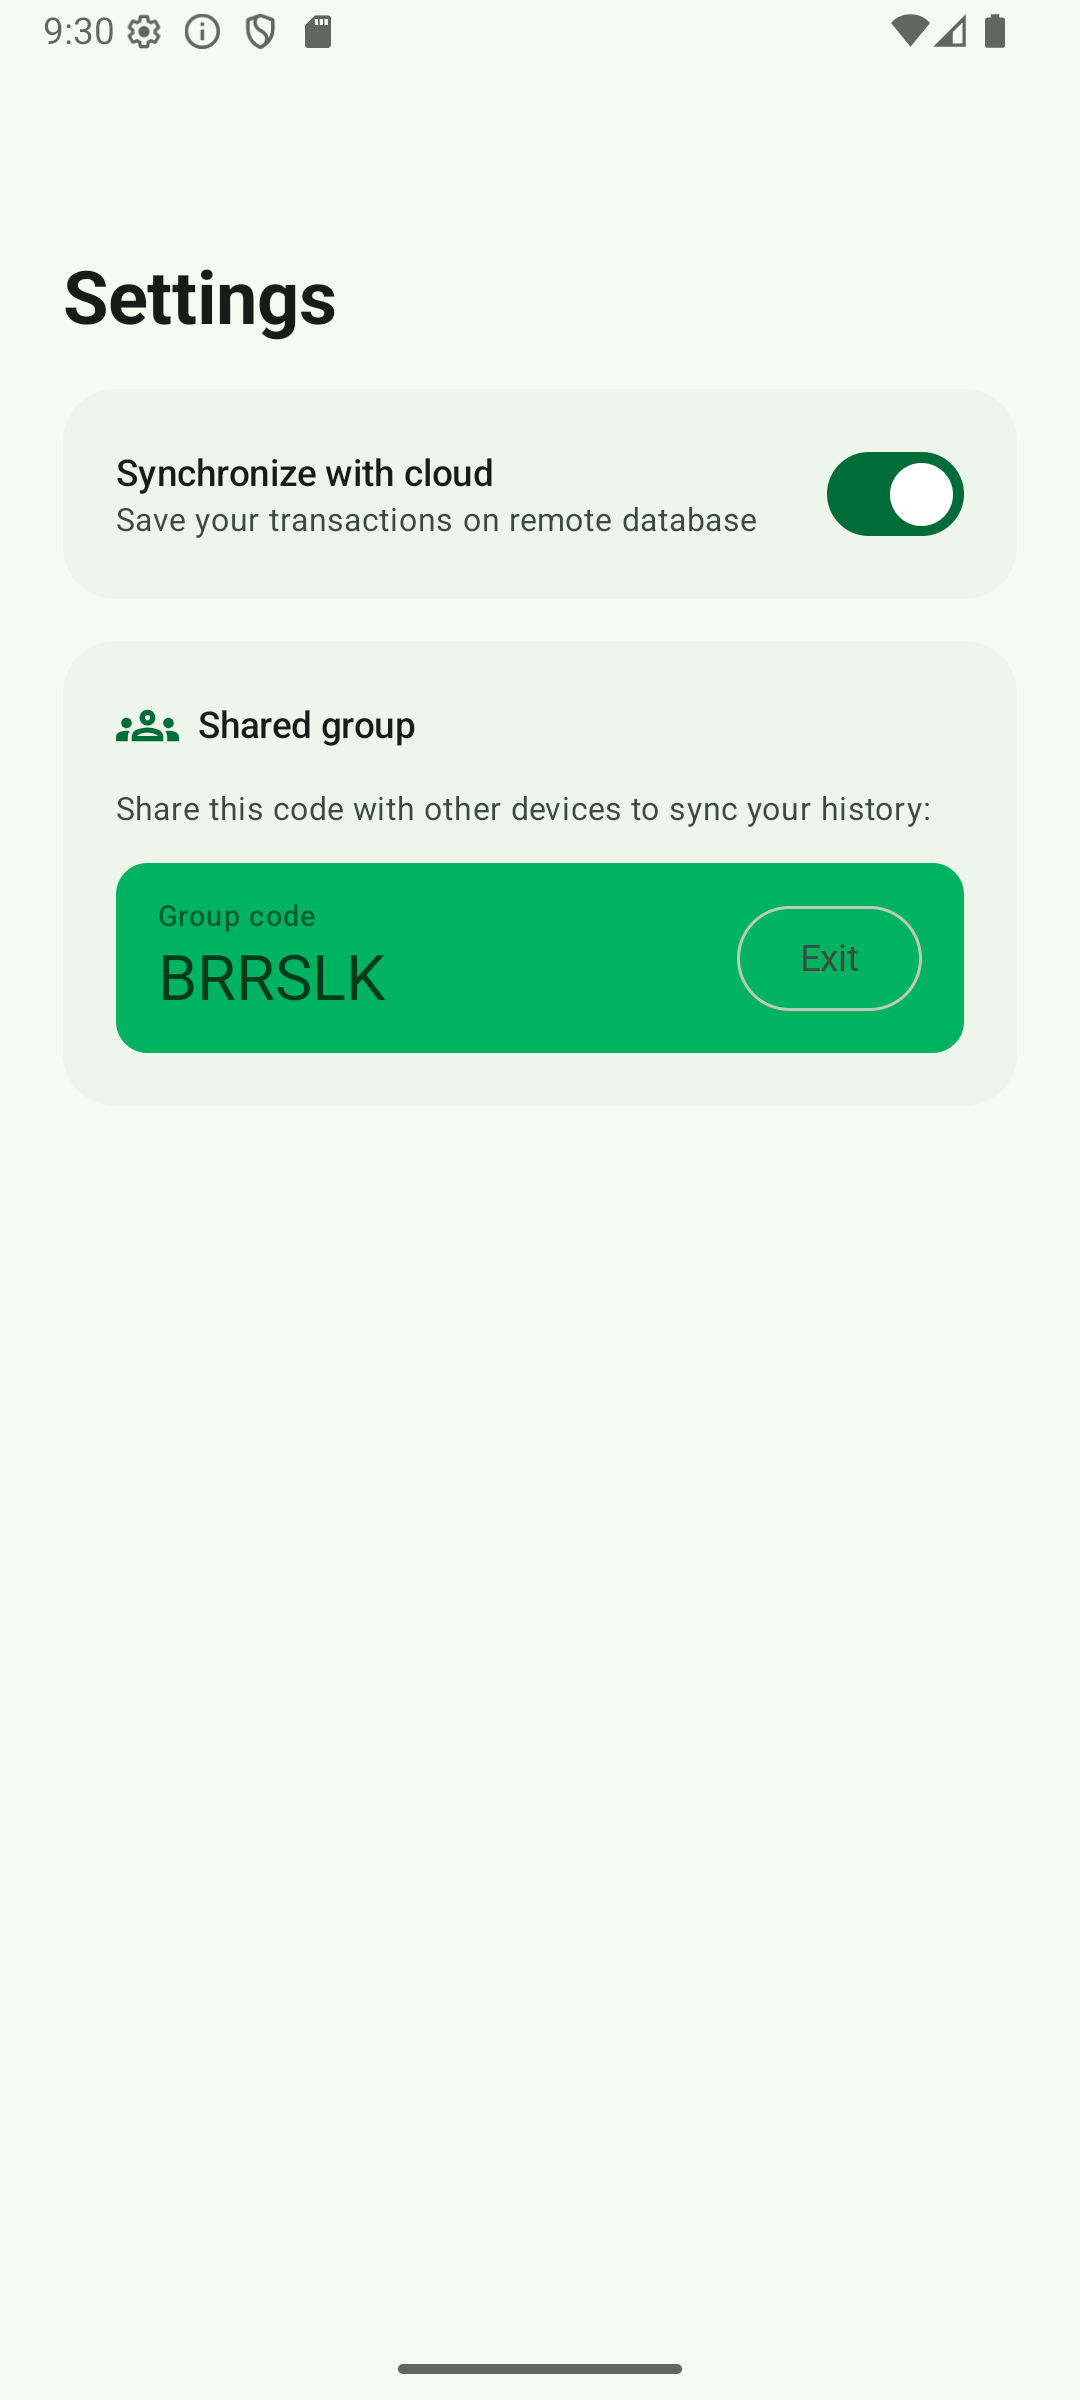
\includegraphics[width=\textwidth]{settings_page_group_created.png}
        \caption{Gruppo creato con codice condivisibile}
        \label{fig:settings-group}
    \end{minipage}
\end{figure}

\clearpage

% ===================== BIBLIOGRAFIA / SITOGRAFIA =====================
\begin{thebibliography}{9}

    \bibitem{doc-repository-progetto}
    Repository pubblica del progetto, \emph{GitHub}.
    \url{https://github.com/sonoAV0/LocalShare}

    \bibitem{doc-WifiDirect}
    Documentazione Wifi-Direct, \emph{Android developers}.
    \url{https://developer.android.com/develop/connectivity/wifi/wifi-direct?hl=it}

    \bibitem{doc-coroutines}
    Documentazione ufficiale coroutines, \emph{Kotlin docs}.
    \url{kotlinlang.org/docs/coroutines-overview.html}

    \bibitem{doc-JWT}
    Documentazione token JWT.
    \url{flask-jwt-extended.readthedocs.io}

    \bibitem{doc-serialization}
    Documentazione kotlinx.serialization, \emph{Kotlin docs}.
    \url{https://kotlinlang.org/docs/serialization.html}

    \bibitem{doc-material3}
    Documentazione Material3, \emph{Android developers}.
    \url{https://developer.android.com/develop/ui/compose/designsystems/material3?hl=it}

    \bibitem{doc-material3-builder}
    Material3 theme builder, \emph{Android developers}.
    \url{https://material-foundation.github.io/material-theme-builder/}

    
\end{thebibliography}



\end{document}
